\documentclass[t]{beamer}
\mode<presentation>

\usepackage{etex}

\usetheme{Madrid}
% other themes: Warsaw, AnnArbor, Antibes, Bergen, Berkeley, Berlin, Boadilla, boxes, CambridgeUS, Copenhagen, Darmstadt, default, Dresden, Frankfurt, Goettingen,
% Hannover, Ilmenau, JuanLesPins, Luebeck, Madrid, Maloe, Marburg, Montpellier, PaloAlto, Pittsburg, Rochester, Singapore, Szeged, classic

\setbeamertemplate{navigation symbols}{\insertslidenavigationsymbol}

\usecolortheme{dolphin}
%\usecolortheme{seagull}
% color themes: albatross, beaver, beetle, crane, default, dolphin, dov, fly, lily, orchid, rose, seagull, seahorse, sidebartab, structure, whale, wolverine

%\usefonttheme{serif}
% font themes: default, professionalfonts, serif, structurebold, structureitalicserif, structuresmallcapsserif

% pdf is displayed in full screen mode automatically
%\hypersetup{pdfpagemode=FullScreen}

%\AtBeginSection[]
%{
%  \begin{frame}<beamer>
%    \frametitle{Outline}
%    \tableofcontents[currentsection,currentsubsection]
%  \end{frame}
%}

% define your own colours:
\definecolor{Red}{rgb}{1,0,0}
\definecolor{Blue}{rgb}{0,0,1}
\definecolor{Green}{rgb}{0,1,0}
\definecolor{magenta}{rgb}{1,0,.6}
\definecolor{lightblue}{rgb}{0,.8,1}
\definecolor{lightpurple}{rgb}{.6,.4,1}
\definecolor{gold}{rgb}{.6,.5,0}
\definecolor{orange}{rgb}{1,0.4,0}
\definecolor{hotpink}{rgb}{1,0,0.5}
\definecolor{newcolor2}{rgb}{.5,.3,.5}
\definecolor{newcolor}{rgb}{0,.3,1}
\definecolor{newcolor3}{rgb}{1,0,.35}
\definecolor{darkgreen1}{rgb}{0, .35, 0}
\definecolor{darkgreen}{rgb}{0, .6, 0}
\definecolor{darkred}{rgb}{.75,0,0}

\xdefinecolor{olive}{cmyk}{0.64,0,0.95,0.4}
\xdefinecolor{purpleish}{cmyk}{0.75,0.75,0,0}

%\usepackage{beamerinnerthemerounded}
% inner themes include circles, default, inmargin, rectangles, rounded

%\usepackage{beamerouterthemesmoothbars}
% outer themes include default, infolines, miniframes, shadow, sidebar, smoothbars, smoothtree, split, tree

\useoutertheme[subsection=false]{smoothbars}

% to have the same footer on all slides
\setbeamertemplate{footline}[text line]{

\includegraphics[height=15pt]{sulogolong.eps}\hfill 
\raisebox{5pt}{Math 207:  Introduction to Statistics}\hfill 
\raisebox{5pt}{Chapter 11: The RMS Error for Regression}\hfill
\raisebox{5pt}{\insertframenumber/\pageref{lastpage}}}
%\setbeamertemplate{footline}[text line]{} % or empty footer

% include packages
\usepackage{subfigure}
\usepackage{multicol}
\usepackage{amsmath}
\usepackage{epsfig}
\usepackage{graphicx}
\usepackage[all,knot]{xy}
\xyoption{arc}
\usepackage{url}
\usepackage{multimedia}
\usepackage{hyperref}
\usepackage{setspace}

\title{Math 207:  Statistics}
\subtitle{Chapter 11:  The RMS Error for Regression}
\author{Ralph Wojtowicz}
\institute{Mathematics Department\\ Shenandoah University}
%\date{\scriptsize 6 February 2012}

\usepackage{pstricks,pst-grad,pst-func,pst-text,pst-node,multido,pst-plot,calc,pst-3dplot}

\newcommand{\BRACE}{
\begin{pspicture}(-3,-2.1)(3,1.1)
\psset{yunit=3,linewidth=0.02}
\psline(-3.5,0)(3.5,0)  
  \psline(-3,0)(-3,-0.04) \rput[t](-3,-0.07){\scriptsize -3\hphantom{-}}
  \psline(-2,0)(-2,-0.04) \rput[t](-2,-0.07){\scriptsize -2\hphantom{-}}
  \psline(-1,0)(-1,-0.04) \rput[t](-1,-0.07){\scriptsize -1\hphantom{-}}
  \psline(0,0)(0,-0.04)   \rput[t](0,-0.07){\scriptsize 0}
  \psline(1,0)(1,-0.04)   \rput[t](1,-0.07){\scriptsize 1}
  \psline(2,0)(2,-0.04)   \rput[t](2,-0.07){\scriptsize 2}
  \psline(3,0)(3,-0.04)   \rput[t](3,-0.07){\scriptsize 3}
  \rput[l](3.6,0){\scriptsize $x$}
\psline(0,0)(0,0.5)
  \psline(-0.12,0.5)(0,0.5)    \rput[r](-0.21,0.5){\scriptsize $0.5$}
  \psline(-0.12,0.25)(0,0.25)  \rput[r](-0.21,0.25){\scriptsize $0.25$}
\psGauss[linecolor=blue,linewidth=0.02,sigma=1,mue=0]{-3}{3}
\pnode(-1,-0.15){A}\pnode(1,-0.15){B}
\psbrace[braceWidth=0.02,braceWidthInner=5pt,braceWidthOuter=5pt](A)(B){\rput{90}(0.25,-0.05){\scriptsize 68\%}}
%
\pnode(-2,-0.15){C}\pnode(2,-0.15){D}
\psbrace[braceWidth=0.02,braceWidthInner=25pt,braceWidthOuter=5pt](C)(D){\rput{90}(0.25,-0.05){\scriptsize 95\%}}
%
\pnode(-3,-0.15){E}\pnode(3,-0.15){F}
\psbrace[braceWidth=0.02,braceWidthInner=45pt,braceWidthOuter=5pt](E)(F){\rput{90}(0.25,-0.1){\scriptsize 99.7\%}}
\end{pspicture}}

\begin{document}

%\frame[plain]{
%	\titlepage
%}


\begin{frame}[plain]
\definecolor{myblue}{rgb}{0,0,0.6}
\definecolor{grayA}{rgb}{0.95,0.95,0.95}
\definecolor{grayB}{rgb}{0.98,0.98,0.98}
\begin{center}

%\begin{pspicture}(0,0)(7,4.8)
\begin{pspicture}(-6,-7)(6,2)
\rput(0,-1.85){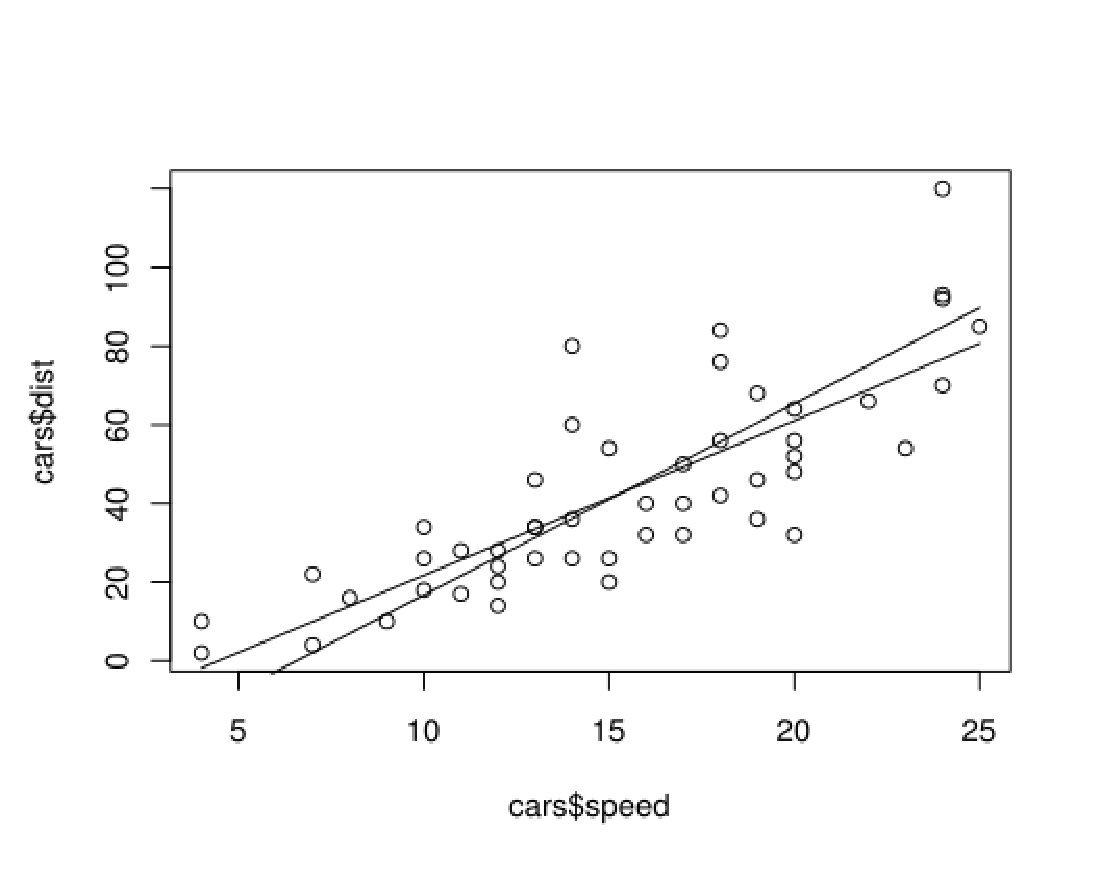
\includegraphics[height=4.2cm,bb=-0 -0 515 350,clip]{CarsRegression.eps}}
\psframe[linewidth=0.02,linecolor=gray](-6.2,-7)(6.2,2.2)
\psframe[linewidth=0.02,linecolor=gray](-6.15,-6.95)(6.15,2.15)
\rput(0,1.4){\color{myblue}\large Math 207:  Introduction to Statistics}
\rput(0,0.6){\color{myblue}Chapter 11:  The RMS Error for Regression}
%\psframebox(0,0)(4,4)
\rput(0,-4.4){\scriptsize Dr.~Ralph Wojtowicz}
%\rput(0,-4.9){\scriptsize CME Department}
\rput(0,-5.6){
\includegraphics[height=2cm]{sulogolong.eps}}
%
%\rput(0,-6.5){\scriptsize 6 February 2012}
\end{pspicture}
\end{center}

\end{frame}

%\section[Outline]{}

\addtocounter{page}{-1}
\addtocounter{framenumber}{-1}

{\footnotesize
\frame{\tableofcontents}
}

\section{RMS Error}
\subsection{Residual Errors}
\begin{frame}[t]\frametitle{The Regression Line}
{\footnotesize 
\begin{itemize}
\item Most points of a scatter plot dont' fall exactly on the regression line.
%   (or any line we might draw to fit the data).
\item The error for a specific point is:
$\displaystyle y_{\mbox{\scriptsize predicted}} \; - \; y_{\mbox{\scriptsize actual}}.$
\item It's the distance between the $y$-value on the line and the 
   $y$-value of the data point.
\end{itemize}

\begin{center}
\begin{pspicture}(0,-0.7)(7,5.0)
\psset{yunit=0.38,dotsize=0.15}
\psdot(1,10)
\psdot(3,9)
\psdot(4,8)
\psdot(4,7)
\psdot(5,1)
\psdot(7,13)
\psline[linewidth=0.02](0,7.8)(7,8.15)(8,8.2)
\rput(3.5,-1.7){$x$}\rput(-1,6.5){$y$}
\psaxes(0,0)(7,13)
%
\psline[linestyle=dotted](7,8.15)(7,13)
\psdot*[linecolor=red](7,8.15)
\rput[l](7,10.575){\ error}
%
\psline[linestyle=dotted](3,7.95)(3,9)
\psdot*[linecolor=red](3,7.95)
\rput[r](3,8.475){error\ }
%
\psline[linestyle=dotted](1,7.85)(1,10)
\psdot*[linecolor=red](1,7.85)
%
\psline[linestyle=dotted](4,8)(4,7)
\psdot*[linecolor=red](4,8)
%
\psline[linestyle=dotted](5,8.05)(5,1)
\psdot*[linecolor=red](5,8.05)
%
\rput(8,5.4){regression line:}
\rput(8,4.5){$y-8\; = \; \frac{1}{20}\,(x - 4)$}
\end{pspicture}
\end{center}}

\end{frame}

\subsection{RMS}
\begin{frame}
\frametitle{The RMS Error for a Line}

\footnotesize
\begin{itemize}
\item Given a scatter plot, the {\color{blue}R.M.S. errror} of a line is 
the root-mean-squared size of the errors:\vspace{-5pt}
\[{\color{blue}\mbox{RMS} = \sqrt{\frac{1}{n}\,\sum_{i=1}^n\,(\mbox{residual error}_i)^2}}\vspace{-3pt}\]
\item It is a measure of the total error of the line that we are using  to fit the data.
\item The regression line is the line that minimizes this error.  
\item The regression line is the \textit{best fit} line.
\item For the regression line, the RMS is:\vspace{-3pt}
\[{\color{darkgreen}\mbox{RMS}_{\mbox{\footnotesize reg}} = \mbox{SD}_y\,\sqrt{1-r^2}}\vspace{-3pt}\]
where $r$ is the correlation and $\mbox{SD}_y$ is the standard deviation of the $y$-values.
\item Notice that:
  \begin{itemize}
\item \scriptsize For a fixed value of $r$, RMS increases with $\mbox{SD}_y$.
\item \scriptsize If $r=1$ or $r=-1$, the RMS is zero (since the points fall exactly on a line).
\item \scriptsize  If $r=0$, then $\mbox{RMS}=\mbox{SD}_y$.
\end{itemize}
\item We have to use the {\color{blue}blue} equation to get RMS if we don't use the regression line.
\end{itemize}

\end{frame}



\section{Examples}
\subsection{Computing RMS}
\begin{frame}
\frametitle{Example:  Regression Line has Minimum RMS}
\newcommand{\Z}{\hphantom{0}}

\footnotesize 

\begin{itemize}
\item For the given $(x,\,y)$ data, find the RMS error for the line $y=x+1$.
\begin{center}
\begin{tabular}{cc|ccc}
$x$ & $y$ & predicted $y$ & error & $\mbox{error}^2$ \\\hline
0   & 1   & 1 & \Z0 & 0\\
1   & 3   & 2 & \Z1 & 1\\
2   & 2   & 3 & $-1$ & 1
\end{tabular}
{\color{blue}$\mbox{RMS} = \sqrt{2/3} = 0.816$}
\end{center}
%
\item<2-> Find the RMS error for the line $y=\frac{3}{2}\,x + 1$
\begin{center}
\begin{tabular}{cc|ccc}
$x$ & $y$ & predicted $y$ & error & $\mbox{error}^2$ \\\hline
0   & 1   & 1 & \Z0 & 0\\
1   & 3   & 5/2 & 1/2 & 1/4\\
2   & 2   & 4 & $-2$ & 4
\end{tabular}
{\color{blue}$\mbox{RMS} = \sqrt{17/12} = 1.19$}
\end{center}
\item<3-> Find the RMS error for the regression line $y=\frac{1}{2}\,x + \frac{3}{2}$
\begin{center}
\begin{tabular}{cc|ccc}
$x$ & $y$ & predicted $y$ & error & $\mbox{error}^2$ \\\hline
0   & 1   & 3/2 & $-1/2$ & 1/4\\
1   & 3   & 2   &  1 & 1\\
2   & 2   & 5/2 & $-1/2$ & 1/4
\end{tabular}
{\color{blue}$\mbox{RMS} = \sqrt{1/2} = 0.707$}
\end{center}
\end{itemize}

\end{frame}

\subsection{Using the RMS Formula}
\begin{frame}
\frametitle{Using the Formula for Regression Line RMS}

\footnotesize

Use the given information and the equation\vspace{-4pt}
\[\mbox{RMS}_{\scriptsize \mbox{reg}} = \mbox{SD}_y\,\sqrt{1-r^2}\vspace{-4pt}\]
to compute the RMS error for the regression line 

  \begin{itemize}
   \item<2-> \footnotesize $\mbox{SD}_y=8$ and $r=\sqrt{3}\,/\,2$\\
      $\mbox{RMS} = 8\,\sqrt{1 - \left(\sqrt{3}\,/2\right)^2} = 
     8\sqrt{1 - 3/4} = 8\sqrt{1/4} = 8\,(1/2) = 4$\vspace{5pt}
%
   \item<3-> \footnotesize $\mbox{SD}_y=1$ and $r=\sqrt{3}\,/\,2$\\
      $\mbox{RMS} = \sqrt{1 - \left(\sqrt{3}\,/2\right)^2} = 
     \sqrt{1 - 3/4} = \sqrt{1/4} = (1/2)$\vspace{5pt}
%
   \item<4-> \footnotesize $\mbox{SD}_y=8$ and $r=0.1$\vspace{3pt}\\
      $\mbox{RMS} = 2\,\sqrt{1 - (0.1)^2} = 
      8\,\sqrt{1 - 0.01} = 8\,\sqrt{0.99}=7.96$\vspace{5pt}
\item<5-> $\mbox{RMS}_{\scriptsize \mbox{reg}}$ increases with $\mbox{SD}_y$.
\item<6-> $\mbox{RMS}_{\scriptsize \mbox{reg}}$ decreases as $r$ approaches $\pm 1$.
\end{itemize}

\end{frame}

\section{Vertical Strips}
\subsection{Vertical Strips}
\begin{frame}
\frametitle{Vertical Strips}
\footnotesize 

\rput(9,-3){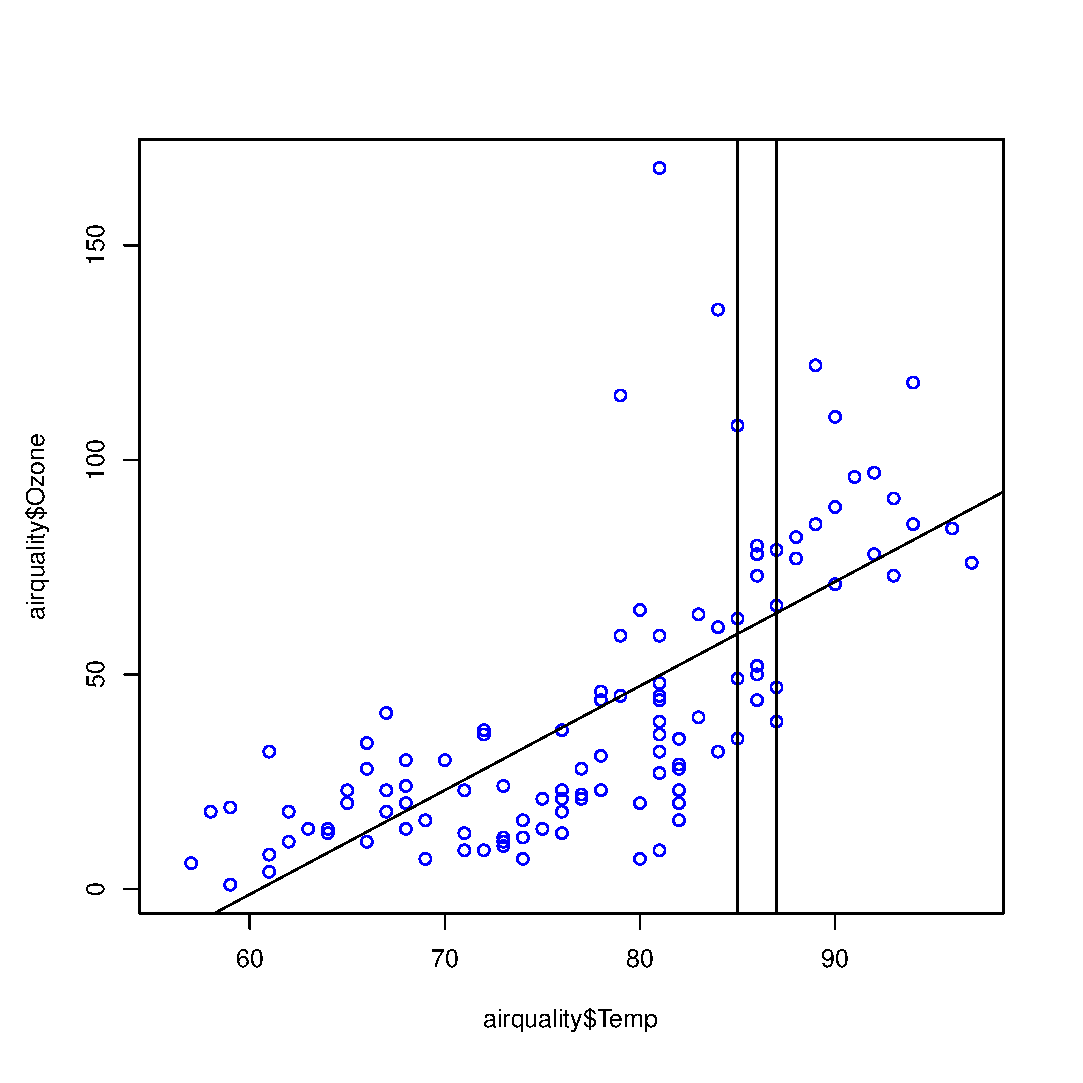
\includegraphics[height=2.5in]{lines.eps}}

\begin{itemize}
\item For each $x$, the $y$-value on\\
      the regression line is the \\
     average of the $y$-values in a\\
      vertical strip.
\item  $y$-values in a strip (approximately)\\
        have a normal distribution with\\
        $\mbox{mean}=y$ value on the line\\
       and $\mbox{SD} = $ the RMS for the\\
        regression line.
\item About 68\% of the points in a strip\\
      are within 1 RMS of the line,  \\
      95\% are withing 2 RMSs, etc.
\end{itemize}
\end{frame}

\subsection{Moving Normal Curves}
\begin{frame}
\frametitle{Moving Normal Curves}

\begin{center}
$\displaystyle \mbox{RMS}_{\scriptsize\mbox{reg}} = \mbox{SD}_y\,\sqrt{1-r^2}$\vspace{3pt}

\scalebox{0.8}{\begin{pspicture}(0,-0.7)(7,6.5)
\psset{yunit=0.5,dotsize=0.15}
\psdot(1,10)
\psdot(3,9)
\psdot(4,8)
\psdot(4,7)
\psdot(5,1)
\psdot(7,13)
\psline[linewidth=0.02](0,7.8)(7,8.15)(8,8.2)
\rput(3.5,-1.7){$x$}\rput(-1,6.5){$y$}
\psaxes(0,0)(7,13)
%
\psdot*[linecolor=red](7,8.15)
     \rput{-90}(7,8.15){\psGauss[sigma=0.6]{-2}{2}}
%
\psdot*[linecolor=red](3,7.95)
     \rput{-90}(3,7.95){\psGauss[sigma=0.6]{-2}{2}}
%
\psdot*[linecolor=red](1,7.85)
     \rput{-90}(1,7.85){\psGauss[sigma=0.6]{-2}{2}}
%
\psdot*[linecolor=red](4,8)
     \rput{-90}(4,8){\psGauss[sigma=0.6]{-2}{2}}
%
\psdot*[linecolor=red](5,8.05)
     \rput{-90}(5,8.05){\psGauss[sigma=0.6]{-2}{2}}
%
\end{pspicture}}
\end{center}

\end{frame}

\subsection{The Normal Curve}
\begin{frame}
\frametitle{Using the Normal Curve}

\footnotesize

For the men age 18--24 in HANES5, the relationship between height and 
weight can be summarized as follows:\vspace{-3pt}
\begin{center}
{\setlength{\tabcolsep}{2pt}\begin{tabular}{rclcrclcc}
average height & $\approx$ & 70 inches, & \hspace{5pt} & SD & $\approx$ & 3 inches,\\
average weight & $\approx$ & 180 pounds, & \hspace{5pt} & SD & $\approx$ & 45 pounds, &
   \hspace{10pt} $r\approx 0.40$\\[-8pt]
\end{tabular}}
\end{center}
\begin{itemize}
\item<2-> Find the equation for the regression line:\vspace{-5pt}
\[{\color{blue}  (y - 180)} = {\color{blue}6\,(x - 70)}\vspace{-8pt}\]
\item<3-> Find the RMS for regression:
\[45\,\sqrt{1 - (0.4)^2} \approx 41.2\;\mbox{pounds}\]
\item<4-> What was the average weight of the 6'2" subjects?
    \[y = 180 + 6\,(74 - 70) = 180 + 24 = 204\;\mbox{pounds}\vspace{-5pt}\]  
\item<5-> About 68\% of the 6'2" subjects had weight in what range?\vspace{-4pt}
 \[204\pm 41.2\;\mbox{pounds}\]
\item<6-> About 95\% of the 6'2" subjects had weight in what range?\vspace{-4pt}
 \[204\pm 2\cdot 41.2 = 204\pm 82.4\;\mbox{pounds}\]
\end{itemize}
\label{lastpage}
\end{frame}

\end{document}
